\chapter{Busca por similaridade}
\label{cap:req}



\begin{overview}
  \lipsum[1]
\end{overview}



\section{Recuperação de Imagens Baseado em Conteúdo}
\label{sec:cbir}

A recuperação de imagem baseada em conteúdo (CBIR) é uma tarefa de grande relevância na área de visão computacional, que consiste em buscar imagens em um banco de dados utilizando características visuais extraídas automaticamente, em vez de depender de metadados ou descrições textuais. O objetivo principal dessa abordagem é identificar imagens visualmente similares à consulta fornecida pelo usuário, considerando atributos como cor, textura, forma ou padrões visuais específicos.

Inicialmente, as técnicas de CBIR baseavam-se em métodos tradicionais de extração de características. Algoritmos como histogramas de cor, transformadas para análise de textura (como Gabor) e detectores de bordas (como Canny) eram amplamente utilizados. Essas abordagens geravam descritores manuais, que eram comparados utilizando métricas de similaridade, como distância euclidiana ou similaridade do cosseno. Apesar de funcionais, esses métodos eram limitados pela incapacidade de capturar características semânticas mais complexas, o que frequentemente resultava em baixa precisão em bancos de dados heterogêneos.

Com os avanços em aprendizado profundo, a utilização de redes neurais convolucionais (Convolutional Neural Networks, CNNs) transformou a abordagem de CBIR. As CNNs possuem a capacidade de aprender representações hierárquicas diretamente dos dados, extraindo características visuais de baixo nível (como bordas) e abstrações de alto nível (como formas e contextos). Essas representações visuais extraídas são codificadas em forma de vetores, também chamados de \emph{embeddings}. Por isso, modelos de aprendizado profundo tornaram-se ferramentas comuns para gerar tais representações visuais das imagens, que podem ser armazenadas e comparadas eficientemente. Essa abordagem não apenas melhora a precisão da recuperação, mas também permite lidar com variações de escala, rotação e iluminação das imagens.

As implementações mais avançadas de CBIR empregam técnicas como aprendizado de métrica e redes neurais siamêsas para otimizar diretamente a tarefa de similaridade visual. Além disso, combinações de embeddings extraídos de CNNs com informações adicionais, como metadados ou descrições textuais, têm sido exploradas para sistemas mais robustos e contextualmente relevantes. Em aplicações complexas, como astronomia ou medicina, onde os bancos de dados são massivos e as diferenças sutis entre imagens são críticas, essas técnicas modernas têm mostrado eficácia superior, tornando a CBIR uma ferramenta essencial para análise de dados e descoberta científica.






\subsection{Métricas de Avaliação da Similaridade}
\label{sec:metricas-sim}

A recuperação de imagens baseada em embeddings gerados por modelos de aprendizado de máquina envolve a comparação de vetores em um espaço latente para determinar a semelhança ou dissimilaridade entre as representações das imagens. Para isso, são amplamente utilizadas métricas de distância ou similaridade, como similaridade do cosseno (Seção \ref{sec:metricas-cos}), produto interno (Seção \ref{sec:metricas-dot}), distância L1 (Seção \ref{sec:metricas-l1}) e distância L2 (Seção \ref{sec:metricas-l2}). Essas métricas capturam diferentes aspectos das relações entre os embeddings e são escolhidas com base nas características do espaço latente e nos objetivos do sistema. Ademais, nessa Seção, também é definida a métrica que quantifica a capacidade preditiva da tarefa de recuperação por similaridade visual na Seção \ref{sec:metricas-map}.


\subsubsection{Distância do Cosseno}
\label{sec:metricas-cos}

A similaridade do cosseno mede o ângulo entre dois vetores no espaço vetorial, desconsiderando suas magnitudes. Ela é amplamente usada em tarefas de recuperação de imagens e processamento de linguagem natural, pois é invariável à escala dos vetores, o que é útil em embeddings que capturam informações relativas às direções no espaço latente.

Formalmente, ela é definida pela eq. \eqref{eq:cos}, onde \( \mathbf{u} \cdot \mathbf{v} \) é o produto interno dos vetores \( \mathbf{u} \) e \( \mathbf{v} \), e \( \|\mathbf{u}\| \) e \( \|\mathbf{v}\| \) são suas normas. Valores de $\cos(\theta)$ variam entre -1 e 1, onde 1 indica vetores perfeitamente alinhados (paralelos), -1 indica vetores opostos, e 0 indica vetores ortogonais. Já a similaridade do cosseno é mais parecida com outras métricas de distância, pois parte do princípio que coisas próximas possuem valores de distância pequenos, variando de 0 a 2. Quanto mais próximo de zero, mais similar.

\begin{equation}\label{eq:cos}
  \text{Similaridade do Cosseno} = 1-\cos(\theta) = 1-\frac{\mathbf{u} \cdot \mathbf{v}}{\|\mathbf{u}\| \|\mathbf{v}\|}
\end{equation}



\subsubsection{Produto Interno}
\label{sec:metricas-dot}

O produto interno é uma métrica simples que mede a projeção de um vetor sobre outro, conforme a eq. \eqref{eq:dot}, onde \( u_i \) e \( v_i \) são as componentes correspondentes dos vetores \( \mathbf{u} \) e \( \mathbf{v} \). Diferentemente da similaridade do cosseno, o produto interno considera tanto a direção quanto a magnitude dos vetores, o que pode ser útil em espaços latentes onde a magnitude dos embeddings também carrega informações relevantes.

\begin{equation}\label{eq:dot}
  \text{Produto Interno} = \mathbf{u} \cdot \mathbf{v} = \sum_{i=1}^n u_i v_i
\end{equation}



\subsubsection{Distância L1}
\label{sec:metricas-l1}
A distância L1, também conhecida como distância de Manhattan, mede a soma das diferenças absolutas entre as componentes correspondentes de dois vetores. Ela é expressa na eq. \eqref{eq:l1}.

Essa métrica é útil em espaços onde as dimensões são interpretadas como contribuições independentes, e variações locais são importantes. A distância L1 tende a ser mais robusta a outliers do que a distância L2, pois considera contribuições lineares de cada dimensão sem elevar as diferenças ao quadrado.

\begin{equation}\label{eq:l1}
  \text{Distância L1} = \|\mathbf{u} - \mathbf{v}\|_1 = \sum_{i=1}^n |u_i - v_i|
\end{equation}


\subsubsection{Distância L2}
\label{sec:metricas-l2}
A distância L2, ou distância Euclidiana, é a métrica mais comum para medir a similaridade entre vetores. Ela calcula a raiz quadrada da soma dos quadrados das diferenças entre as componentes correspondentes dos vetores, conforme a eq. \eqref{eq:l2}.

Esta métrica é amplamente utilizada devido à sua interpretação geométrica intuitiva como a distância direta entre dois pontos em um espaço multidimensional. No entanto, ela é sensível a outliers, pois penaliza diferenças grandes mais severamente do que a distância L1.

\begin{equation}\label{eq:l2}
  \text{Distância L2} = \|\mathbf{u} - \mathbf{v}\|_2 = \sqrt{\sum_{i=1}^n (u_i - v_i)^2}
\end{equation}





\subsubsection{Métrica de Desempenho da Busca}
\label{sec:metricas-map}
A métrica mAP (mean Average Precision) é amplamente utilizada para avaliar o desempenho de sistemas de recuperação de informações, incluindo a recuperação de imagens baseada em embeddings gerados por modelos de aprendizado de máquina. Essa métrica combina precisão e revocação em um único valor, fornecendo uma medida robusta da capacidade de um modelo em recuperar itens relevantes em tarefas onde a ordenação dos resultados importa.

O cálculo do mAP começa pela definição da \emph{Average Precision} (AP), que mede a precisão média em diferentes níveis de revocação para um conjunto de resultados ordenados. Em um cenário típico de recuperação, para cada consulta, o sistema retorna uma lista ordenada de itens, e o objetivo é avaliar como os itens relevantes estão distribuídos ao longo dessa lista. Dessa forma, para uma consulta \( q \), a AP é definida pela eq. \eqref{eq:ap}, onde \( N \) é o número total de itens retornados; \( P(k) \) é a precisão até a posição \( k \) na lista de resultados; e \( rel(k) \) é uma função indicadora que vale 1 se o item na posição \( k \) for relevante e 0 caso contrário.

\begin{equation}\label{eq:ap}
  AP(q) = \frac{\sum_{k=1}^N P(k) \cdot rel(k)}{\text{Total de itens relevantes}}
\end{equation}

Intuitivamente, a AP calcula a média das precisões em cada ponto onde um item relevante é encontrado, ponderando pela relevância. Isso recompensa sistemas que colocam itens relevantes nas primeiras posições, refletindo a importância da ordenação.

A métrica mAP é obtida como a média da AP sobre todas as consultas \( Q \), conforme a eq. \eqref{eq:map}, onde \( |Q| \) é o número total de consultas. Esse valor sintetiza o desempenho global do sistema, considerando tanto a qualidade das predições individuais quanto a consistência do modelo em diferentes consultas.

\begin{equation}\label{eq:map}
  mAP = \frac{1}{|Q|} \sum_{q \in Q} AP(q)
\end{equation}

O mAP é mais informativo que métricas como acurácia ou precisão isolada, pois considera explicitamente a ordenação dos resultados e é adequado para sistemas de recuperação onde o número de itens relevantes por consulta pode variar. Além disso, o mAP não é influenciado por classes desbalanceadas, pois avalia separadamente a qualidade da recuperação para cada consulta.







\section{Avaliação da Recuperação de Imagens}
\label{sec:res-ret}

A avaliação quantitativa do desempenho do sistema para a tarefa de recuperação de imagens é feita utilizando a métrica mean Average Precision (mAP; Seção \ref{sec:metricas-map}), pois esta medida é crucial para avaliar a capacidade do sistema em priorizar e classificar corretamente imagens relevantes em relação a consultas específicas. A mAP integra a precisão ao longo de diferentes níveis de revocação, proporcionando uma visão detalhada do desempenho global do modelo em recuperar galáxias em grandes bancos de dados.

Os valores de mAP apresentados na Tabela \ref{tab:test-map} evidenciam a habilidade do modelo em manter alta relevância entre os itens recuperados, mesmo em cenários de grande complexidade ou com classes desbalanceadas. Essa métrica assegura que o sistema não apenas é eficaz em identificar galáxias relevantes, mas também organiza as recuperações de forma a maximizar sua utilidade científica, destacando a robustez e a capacidade de generalização do modelo para aplicações astronômicas.

\begin{table}[!ht]
  \centering
  \caption{Avaliação do modelo para tarefa de recuperação de imagens}
  \label{tab:test-map}
  \begin{tabular}{lc}
    \toprule
    Questão            & mAP      \\
    \midrule
    Spiral winding     & 0.988254 \\
    Bar                & 0.980521 \\
    Edge on bulge      & 0.990124 \\
    Disk edge on       & 0.999986 \\
    Smooth or featured & 0.987412 \\
    Has spiral arms    & 0.968340 \\
    Galaxy Symetrical  & 0.962513 \\
    Clumpy appearence  & 0.957814 \\
    How rounded        & 0.978536 \\
    Merging            & 0.963656 \\
    Bulge size         & 0.987431 \\
    Spiral arms count  & 0.960259 \\
    \bottomrule
  \end{tabular}
\end{table}


A seguir, as Figs. \ref{fig:q1}, \ref{fig:q2}, \ref{fig:q3}, \ref{fig:q4}, \ref{fig:q5}, \ref{fig:q6} e \ref{fig:q7} mostram as buscas por similaridade visual para vários tipos de galáxias com a finalidade de exemplificar os resultados das buscas por similaridade visual obtidas pelo sistema desenvolvido.


\begin{figure}[!ht]
  \centering
  \caption{Resultados da busca para a galáxia UGC 9010}
  \label{fig:q1}
  \begin{overpic}[width=0.194\linewidth]{figures/stamps/q1_0}
    \put (3, 7) {\large\color{white} Query}
  \end{overpic}
  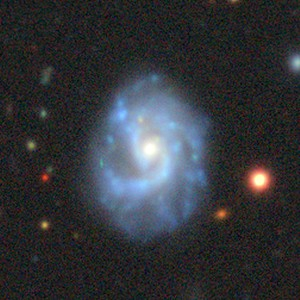
\includegraphics[width=0.194\linewidth]{figures/stamps/q1_1}
  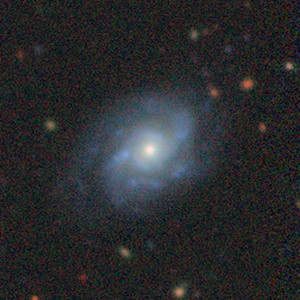
\includegraphics[width=0.194\linewidth]{figures/stamps/q1_2}
  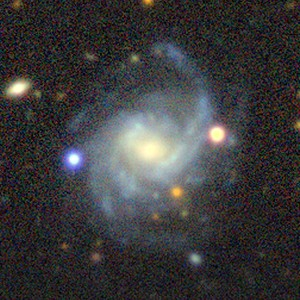
\includegraphics[width=0.194\linewidth]{figures/stamps/q1_3}
  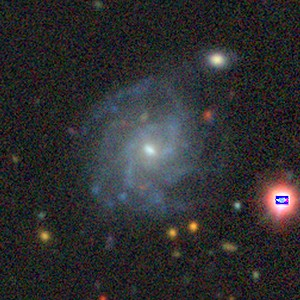
\includegraphics[width=0.194\linewidth]{figures/stamps/q1_4}\\[2mm]
  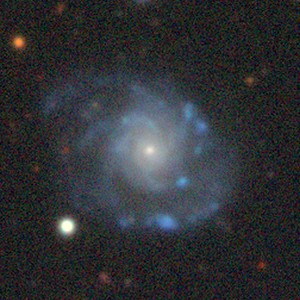
\includegraphics[width=0.194\linewidth]{figures/stamps/q1_5}
  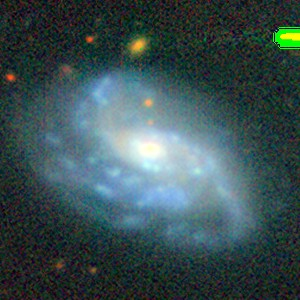
\includegraphics[width=0.194\linewidth]{figures/stamps/q1_6}
  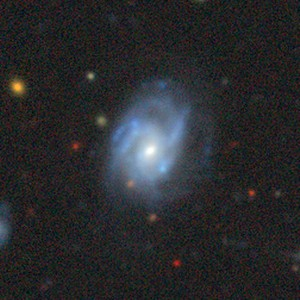
\includegraphics[width=0.194\linewidth]{figures/stamps/q1_7}
  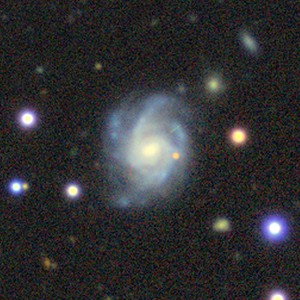
\includegraphics[width=0.194\linewidth]{figures/stamps/q1_8}
  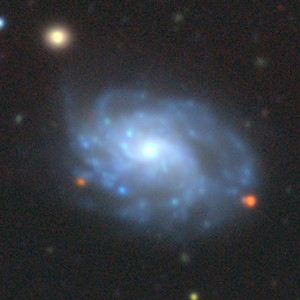
\includegraphics[width=0.194\linewidth]{figures/stamps/q1_9}\\[2mm]
  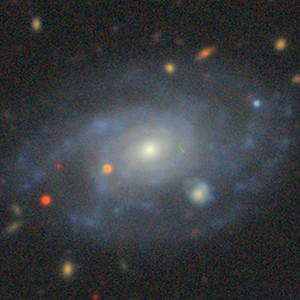
\includegraphics[width=0.194\linewidth]{figures/stamps/q1_10}
  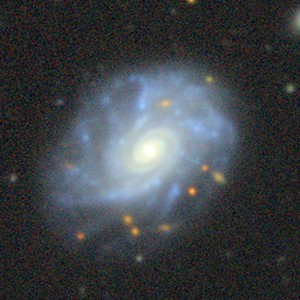
\includegraphics[width=0.194\linewidth]{figures/stamps/q1_11}
  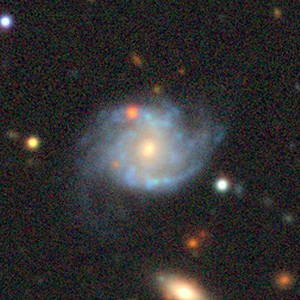
\includegraphics[width=0.194\linewidth]{figures/stamps/q1_12}
  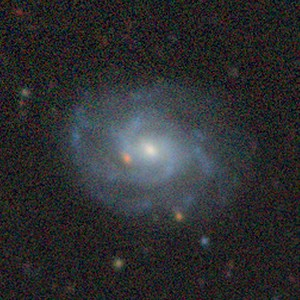
\includegraphics[width=0.194\linewidth]{figures/stamps/q1_13}
  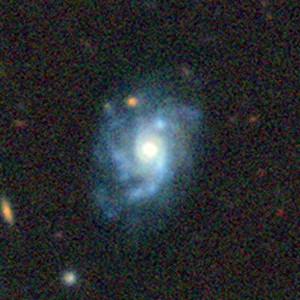
\includegraphics[width=0.194\linewidth]{figures/stamps/q1_14}\\[2mm]
  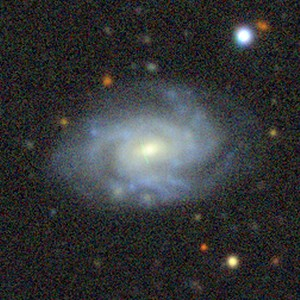
\includegraphics[width=0.194\linewidth]{figures/stamps/q1_15}
  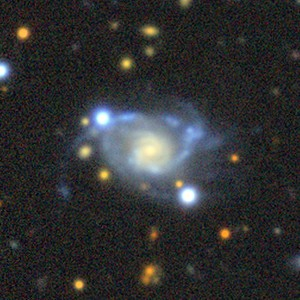
\includegraphics[width=0.194\linewidth]{figures/stamps/q1_16}
  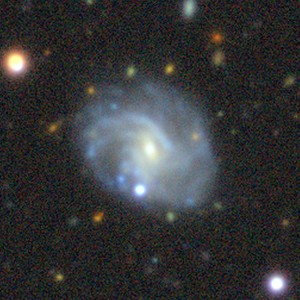
\includegraphics[width=0.194\linewidth]{figures/stamps/q1_17}
  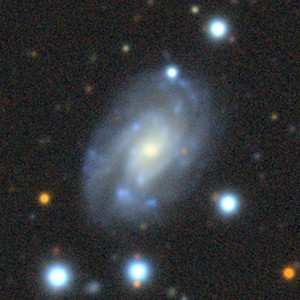
\includegraphics[width=0.194\linewidth]{figures/stamps/q1_18}
  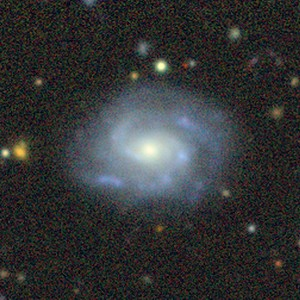
\includegraphics[width=0.194\linewidth]{figures/stamps/q1_19}\\[2mm]
  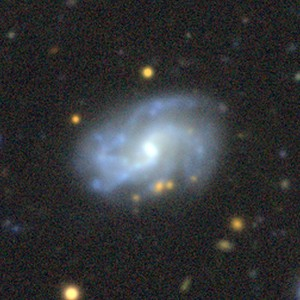
\includegraphics[width=0.194\linewidth]{figures/stamps/q1_20}
  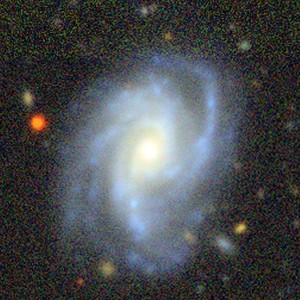
\includegraphics[width=0.194\linewidth]{figures/stamps/q1_21}
  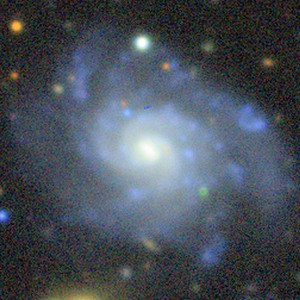
\includegraphics[width=0.194\linewidth]{figures/stamps/q1_22}
  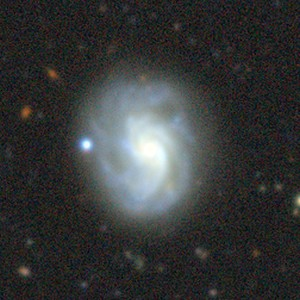
\includegraphics[width=0.194\linewidth]{figures/stamps/q1_23}
  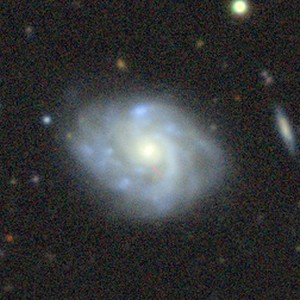
\includegraphics[width=0.194\linewidth]{figures/stamps/q1_24}\\[2mm]
  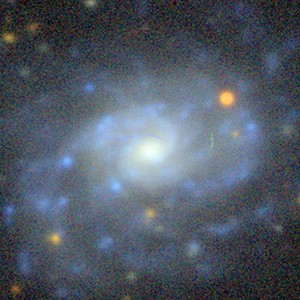
\includegraphics[width=0.194\linewidth]{figures/stamps/q1_25}
  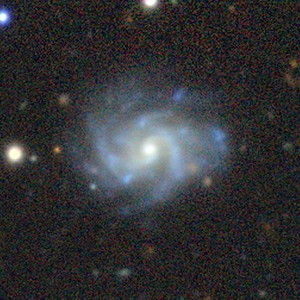
\includegraphics[width=0.194\linewidth]{figures/stamps/q1_26}
  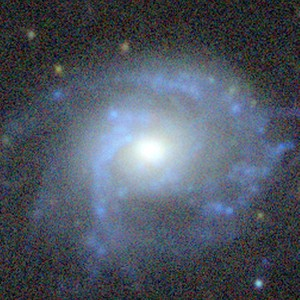
\includegraphics[width=0.194\linewidth]{figures/stamps/q1_27}
  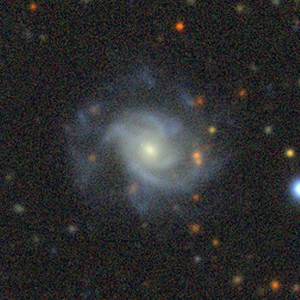
\includegraphics[width=0.194\linewidth]{figures/stamps/q1_28}
  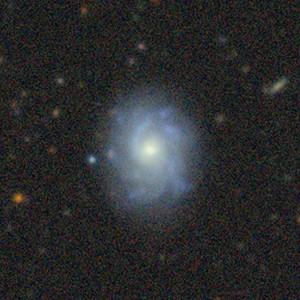
\includegraphics[width=0.194\linewidth]{figures/stamps/q1_29}
  \legend{UGC 9010 é uma galáxia espiral com orientação face-on (face para o observador). O primeiro painel (Query) mostra a imagem da galáxia UGC 9010, utilizada como referência. Os demais painéis mostram as galáxias obtidas por similaridade visual. Esta busca utilizou a distância do cosseno (Seção \ref{sec:metricas-cos}) como métrica de similaridade.}
\end{figure}


\begin{figure}[!ht]
  \centering
  \caption{Resultados da busca para a galáxia NGC 1043}
  \label{fig:q2}
  \begin{overpic}[width=0.194\linewidth]{figures/stamps/q2_0}
    \put (3, 7) {\large\color{white} Query}
  \end{overpic}
  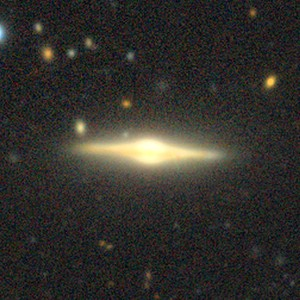
\includegraphics[width=0.194\linewidth]{figures/stamps/q2_1}
  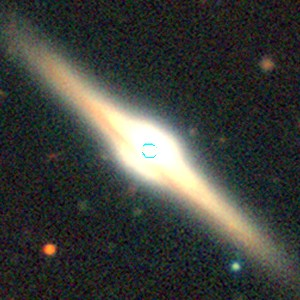
\includegraphics[width=0.194\linewidth]{figures/stamps/q2_2}
  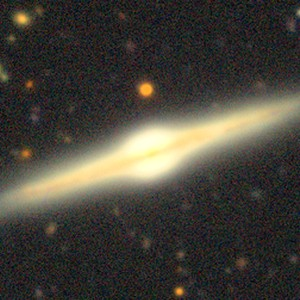
\includegraphics[width=0.194\linewidth]{figures/stamps/q2_3}
  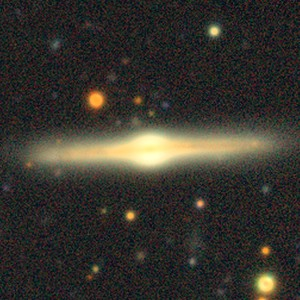
\includegraphics[width=0.194\linewidth]{figures/stamps/q2_4}\\[2mm]
  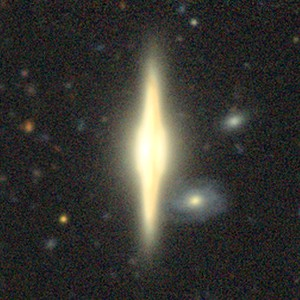
\includegraphics[width=0.194\linewidth]{figures/stamps/q2_5}
  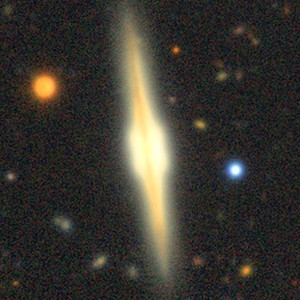
\includegraphics[width=0.194\linewidth]{figures/stamps/q2_6}
  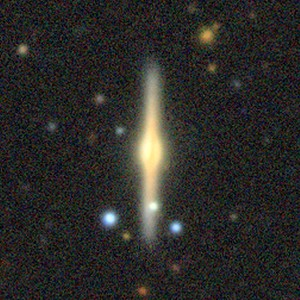
\includegraphics[width=0.194\linewidth]{figures/stamps/q2_7}
  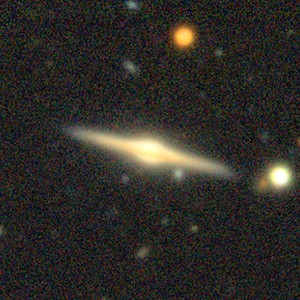
\includegraphics[width=0.194\linewidth]{figures/stamps/q2_8}
  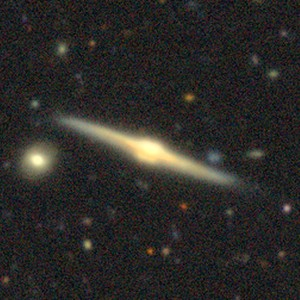
\includegraphics[width=0.194\linewidth]{figures/stamps/q2_9}\\[2mm]
  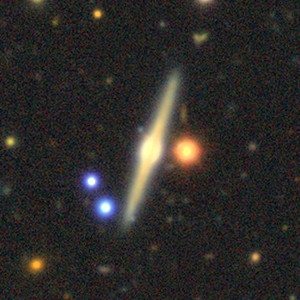
\includegraphics[width=0.194\linewidth]{figures/stamps/q2_10}
  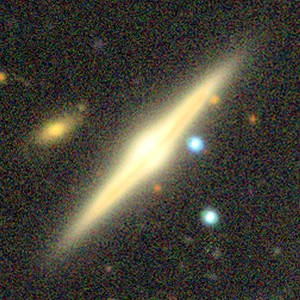
\includegraphics[width=0.194\linewidth]{figures/stamps/q2_11}
  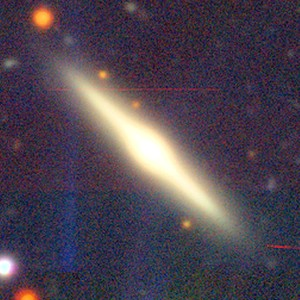
\includegraphics[width=0.194\linewidth]{figures/stamps/q2_12}
  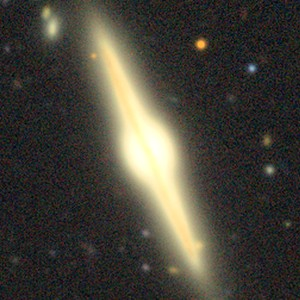
\includegraphics[width=0.194\linewidth]{figures/stamps/q2_13}
  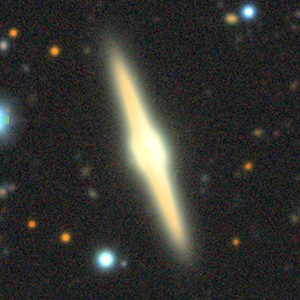
\includegraphics[width=0.194\linewidth]{figures/stamps/q2_14}\\[2mm]
  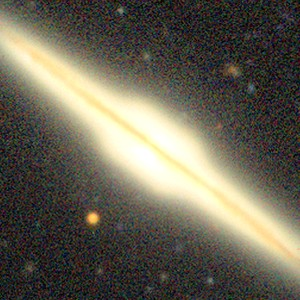
\includegraphics[width=0.194\linewidth]{figures/stamps/q2_15}
  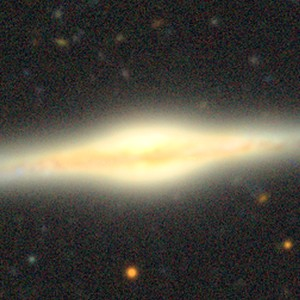
\includegraphics[width=0.194\linewidth]{figures/stamps/q2_16}
  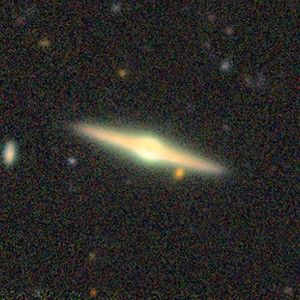
\includegraphics[width=0.194\linewidth]{figures/stamps/q2_17}
  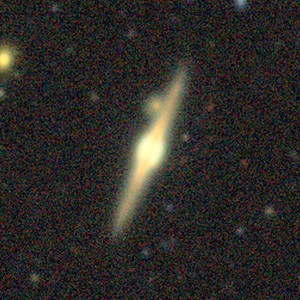
\includegraphics[width=0.194\linewidth]{figures/stamps/q2_18}
  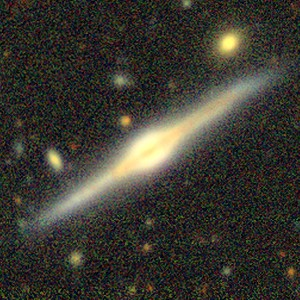
\includegraphics[width=0.194\linewidth]{figures/stamps/q2_19}\\[2mm]
  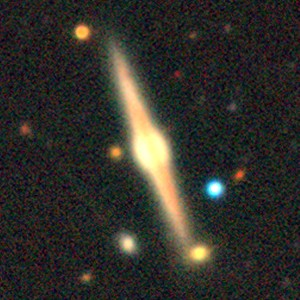
\includegraphics[width=0.194\linewidth]{figures/stamps/q2_20}
  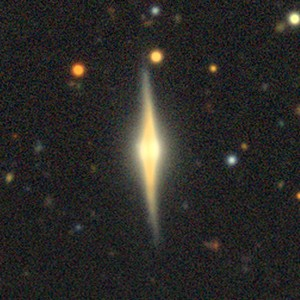
\includegraphics[width=0.194\linewidth]{figures/stamps/q2_21}
  \includegraphics[width=0.194\linewidth]{figures/stamps/q2_22}
  \includegraphics[width=0.194\linewidth]{figures/stamps/q2_23}
  \includegraphics[width=0.194\linewidth]{figures/stamps/q2_24}\\[2mm]
  \includegraphics[width=0.194\linewidth]{figures/stamps/q2_25}
  \includegraphics[width=0.194\linewidth]{figures/stamps/q2_26}
  \includegraphics[width=0.194\linewidth]{figures/stamps/q2_27}
  \includegraphics[width=0.194\linewidth]{figures/stamps/q2_28}
  \includegraphics[width=0.194\linewidth]{figures/stamps/q2_29}
  \legend{NGC 1043 é uma galáxia espiral com orientação edge-on (borda para o observador). O primeiro painel (Query) mostra a imagem da galáxia NGC 1043, utilizada como referência. Os demais painéis mostram as galáxias obtidas por similaridade visual. Esta busca utilizou a distância do cosseno (Seção \ref{sec:metricas-cos}) como métrica de similaridade.}
\end{figure}



\begin{figure}[!ht]
  \centering
  \caption{Resultados da busca para a galáxia J082404.58+315023.3}
  \label{fig:q3}
  \begin{overpic}[width=0.194\linewidth]{figures/stamps/q3_0}
    \put (3, 7) {\large\color{white} Query}
  \end{overpic}
  \includegraphics[width=0.194\linewidth]{figures/stamps/q3_1}
  \includegraphics[width=0.194\linewidth]{figures/stamps/q3_2}
  \includegraphics[width=0.194\linewidth]{figures/stamps/q3_3}
  \includegraphics[width=0.194\linewidth]{figures/stamps/q3_4}\\[2mm]
  \includegraphics[width=0.194\linewidth]{figures/stamps/q3_5}
  \includegraphics[width=0.194\linewidth]{figures/stamps/q3_6}
  \includegraphics[width=0.194\linewidth]{figures/stamps/q3_7}
  \includegraphics[width=0.194\linewidth]{figures/stamps/q3_8}
  \includegraphics[width=0.194\linewidth]{figures/stamps/q3_9}\\[2mm]
  \includegraphics[width=0.194\linewidth]{figures/stamps/q3_10}
  \includegraphics[width=0.194\linewidth]{figures/stamps/q3_11}
  \includegraphics[width=0.194\linewidth]{figures/stamps/q3_12}
  \includegraphics[width=0.194\linewidth]{figures/stamps/q3_13}
  \includegraphics[width=0.194\linewidth]{figures/stamps/q3_14}\\[2mm]
  \includegraphics[width=0.194\linewidth]{figures/stamps/q3_15}
  \includegraphics[width=0.194\linewidth]{figures/stamps/q3_16}
  \includegraphics[width=0.194\linewidth]{figures/stamps/q3_17}
  \includegraphics[width=0.194\linewidth]{figures/stamps/q3_18}
  \includegraphics[width=0.194\linewidth]{figures/stamps/q3_19}\\[2mm]
  \includegraphics[width=0.194\linewidth]{figures/stamps/q3_20}
  \includegraphics[width=0.194\linewidth]{figures/stamps/q3_21}
  \includegraphics[width=0.194\linewidth]{figures/stamps/q3_22}
  \includegraphics[width=0.194\linewidth]{figures/stamps/q3_23}
  \includegraphics[width=0.194\linewidth]{figures/stamps/q3_24}\\[2mm]
  \includegraphics[width=0.194\linewidth]{figures/stamps/q3_25}
  \includegraphics[width=0.194\linewidth]{figures/stamps/q3_26}
  \includegraphics[width=0.194\linewidth]{figures/stamps/q3_27}
  \includegraphics[width=0.194\linewidth]{figures/stamps/q3_28}
  \includegraphics[width=0.194\linewidth]{figures/stamps/q3_29}
  \legend{J082404.58+315023.3 é uma galáxia compacta, sua ocorrência na natureza é extremamente rara. O primeiro painel (Query) mostra a imagem da galáxia J082404.58+315023.3, utilizada como referência. Os demais painéis mostram as galáxias obtidas por similaridade visual. Esta busca utilizou a distância do cosseno (Seção \ref{sec:metricas-cos}) como métrica de similaridade.}
\end{figure}



\begin{figure}[!ht]
  \centering
  \caption{Resultados da busca para a galáxia UGC 1698}
  \label{fig:q4}
  \begin{overpic}[width=0.194\linewidth]{figures/stamps/q4_0}
    \put (3, 7) {\large\color{white} Query}
  \end{overpic}
  \includegraphics[width=0.194\linewidth]{figures/stamps/q4_1}
  \includegraphics[width=0.194\linewidth]{figures/stamps/q4_7}
  \includegraphics[width=0.194\linewidth]{figures/stamps/q4_3}
  \includegraphics[width=0.194\linewidth]{figures/stamps/q4_4}\\[2mm]
  \includegraphics[width=0.194\linewidth]{figures/stamps/q4_5}
  \includegraphics[width=0.194\linewidth]{figures/stamps/q4_6}
  \includegraphics[width=0.194\linewidth]{figures/stamps/q4_2}
  \includegraphics[width=0.194\linewidth]{figures/stamps/q4_8}
  \includegraphics[width=0.194\linewidth]{figures/stamps/q4_9}\\[2mm]
  \includegraphics[width=0.194\linewidth]{figures/stamps/q4_10}
  \includegraphics[width=0.194\linewidth]{figures/stamps/q4_11}
  \includegraphics[width=0.194\linewidth]{figures/stamps/q4_12}
  \includegraphics[width=0.194\linewidth]{figures/stamps/q4_21}
  \includegraphics[width=0.194\linewidth]{figures/stamps/q4_14}\\[2mm]
  \includegraphics[width=0.194\linewidth]{figures/stamps/q4_15}
  \includegraphics[width=0.194\linewidth]{figures/stamps/q4_16}
  \includegraphics[width=0.194\linewidth]{figures/stamps/q4_17}
  \includegraphics[width=0.194\linewidth]{figures/stamps/q4_18}
  \includegraphics[width=0.194\linewidth]{figures/stamps/q4_19}\\[2mm]
  \includegraphics[width=0.194\linewidth]{figures/stamps/q4_20}
  \includegraphics[width=0.194\linewidth]{figures/stamps/q4_13}
  \includegraphics[width=0.194\linewidth]{figures/stamps/q4_22}
  \includegraphics[width=0.194\linewidth]{figures/stamps/q4_23}
  \includegraphics[width=0.194\linewidth]{figures/stamps/q4_24}\\[2mm]
  \includegraphics[width=0.194\linewidth]{figures/stamps/q4_25}
  \includegraphics[width=0.194\linewidth]{figures/stamps/q4_26}
  \includegraphics[width=0.194\linewidth]{figures/stamps/q4_27}
  \includegraphics[width=0.194\linewidth]{figures/stamps/q4_28}
  \includegraphics[width=0.194\linewidth]{figures/stamps/q4_29}
  \legend{UGC 1698 é uma espiral barrada, o sistema foi capaz de recuperar galáxias muito parecidas. O primeiro painel (Query) mostra a imagem da galáxia UGC 1698, utilizada como referência. Os demais painéis mostram as galáxias obtidas por similaridade visual. Esta busca utilizou a distância do cosseno (Seção \ref{sec:metricas-cos}) como métrica de similaridade.}
\end{figure}





\begin{figure}[!ht]
  \centering
  \caption{Resultados da busca para a galáxia J060430.95-470755.7}
  \label{fig:q5}
  \begin{overpic}[width=0.194\linewidth]{figures/stamps/q5_0}
    \put (3, 7) {\large\color{white} Query}
  \end{overpic}
  \includegraphics[width=0.194\linewidth]{figures/stamps/q5_1}
  \includegraphics[width=0.194\linewidth]{figures/stamps/q5_2}
  \includegraphics[width=0.194\linewidth]{figures/stamps/q5_3}
  \includegraphics[width=0.194\linewidth]{figures/stamps/q5_4}\\[2mm]
  \includegraphics[width=0.194\linewidth]{figures/stamps/q5_5}
  \includegraphics[width=0.194\linewidth]{figures/stamps/q5_6}
  \includegraphics[width=0.194\linewidth]{figures/stamps/q5_7}
  \includegraphics[width=0.194\linewidth]{figures/stamps/q5_8}
  \includegraphics[width=0.194\linewidth]{figures/stamps/q5_9}\\[2mm]
  \includegraphics[width=0.194\linewidth]{figures/stamps/q5_10}
  \includegraphics[width=0.194\linewidth]{figures/stamps/q5_11}
  \includegraphics[width=0.194\linewidth]{figures/stamps/q5_12}
  \includegraphics[width=0.194\linewidth]{figures/stamps/q5_13}
  \includegraphics[width=0.194\linewidth]{figures/stamps/q5_14}\\[2mm]
  \includegraphics[width=0.194\linewidth]{figures/stamps/q5_15}
  \includegraphics[width=0.194\linewidth]{figures/stamps/q5_16}
  \includegraphics[width=0.194\linewidth]{figures/stamps/q5_17}
  \includegraphics[width=0.194\linewidth]{figures/stamps/q5_18}
  \includegraphics[width=0.194\linewidth]{figures/stamps/q5_19}\\[2mm]
  \includegraphics[width=0.194\linewidth]{figures/stamps/q5_20}
  \includegraphics[width=0.194\linewidth]{figures/stamps/q5_21}
  \includegraphics[width=0.194\linewidth]{figures/stamps/q5_22}
  \includegraphics[width=0.194\linewidth]{figures/stamps/q5_23}
  \includegraphics[width=0.194\linewidth]{figures/stamps/q5_24}\\[2mm]
  \includegraphics[width=0.194\linewidth]{figures/stamps/q5_25}
  \includegraphics[width=0.194\linewidth]{figures/stamps/q5_26}
  \includegraphics[width=0.194\linewidth]{figures/stamps/q5_27}
  \includegraphics[width=0.194\linewidth]{figures/stamps/q5_28}
  \includegraphics[width=0.194\linewidth]{figures/stamps/q5_29}
  \legend{J060430.95-470755.7 é uma galáxia com enrolamento dos braços espirais abertos. O primeiro painel (Query) mostra a imagem da galáxia J060430.95-470755.7, utilizada como referência. Os demais painéis mostram as galáxias obtidas por similaridade visual. Esta busca utilizou a distância do cosseno (Seção \ref{sec:metricas-cos}) como métrica de similaridade.}
\end{figure}




\begin{figure}[!ht]
  \centering
  \caption{Resultados da busca para a galáxia UGC 767}
  \label{fig:q6}
  \begin{overpic}[width=0.194\linewidth]{figures/stamps/q6_0}
    \put (3, 7) {\large\color{white} Query}
  \end{overpic}
  \includegraphics[width=0.194\linewidth]{figures/stamps/q6_1}
  \includegraphics[width=0.194\linewidth]{figures/stamps/q6_2}
  \includegraphics[width=0.194\linewidth]{figures/stamps/q6_3}
  \includegraphics[width=0.194\linewidth]{figures/stamps/q6_4}\\[2mm]
  \includegraphics[width=0.194\linewidth]{figures/stamps/q6_5}
  \includegraphics[width=0.194\linewidth]{figures/stamps/q6_6}
  \includegraphics[width=0.194\linewidth]{figures/stamps/q6_7}
  \includegraphics[width=0.194\linewidth]{figures/stamps/q6_8}
  \includegraphics[width=0.194\linewidth]{figures/stamps/q6_9}\\[2mm]
  \includegraphics[width=0.194\linewidth]{figures/stamps/q6_10}
  \includegraphics[width=0.194\linewidth]{figures/stamps/q6_11}
  \includegraphics[width=0.194\linewidth]{figures/stamps/q6_12}
  \includegraphics[width=0.194\linewidth]{figures/stamps/q6_13}
  \includegraphics[width=0.194\linewidth]{figures/stamps/q6_14}\\[2mm]
  \includegraphics[width=0.194\linewidth]{figures/stamps/q6_15}
  \includegraphics[width=0.194\linewidth]{figures/stamps/q6_16}
  \includegraphics[width=0.194\linewidth]{figures/stamps/q6_17}
  \includegraphics[width=0.194\linewidth]{figures/stamps/q6_18}
  \includegraphics[width=0.194\linewidth]{figures/stamps/q6_19}\\[2mm]
  \includegraphics[width=0.194\linewidth]{figures/stamps/q6_20}
  \includegraphics[width=0.194\linewidth]{figures/stamps/q6_21}
  \includegraphics[width=0.194\linewidth]{figures/stamps/q6_22}
  \includegraphics[width=0.194\linewidth]{figures/stamps/q6_23}
  \includegraphics[width=0.194\linewidth]{figures/stamps/q6_24}\\[2mm]
  \includegraphics[width=0.194\linewidth]{figures/stamps/q6_25}
  \includegraphics[width=0.194\linewidth]{figures/stamps/q6_26}
  \includegraphics[width=0.194\linewidth]{figures/stamps/q6_27}
  \includegraphics[width=0.194\linewidth]{figures/stamps/q6_28}
  \includegraphics[width=0.194\linewidth]{figures/stamps/q6_29}
  \legend{UGC 767 é uma galáxia elíptica. O primeiro painel (Query) mostra a imagem da galáxia UGC 767, utilizada como referência. Os demais painéis mostram as galáxias obtidas por similaridade visual. Esta busca utilizou a distância do cosseno (Seção \ref{sec:metricas-cos}) como métrica de similaridade.}
\end{figure}



\begin{figure}[!ht]
  \centering
  \caption{Resultados da busca para a galáxia J151806.13+424445.2}
  \label{fig:q7}
  \begin{overpic}[width=0.194\linewidth]{figures/stamps/q7_0}
    \put (3, 7) {\large\color{white} Query}
  \end{overpic}
  \includegraphics[width=0.194\linewidth]{figures/stamps/q7_1}
  \includegraphics[width=0.194\linewidth]{figures/stamps/q7_2}
  \includegraphics[width=0.194\linewidth]{figures/stamps/q7_3}
  \includegraphics[width=0.194\linewidth]{figures/stamps/q7_4}\\[2mm]
  \includegraphics[width=0.194\linewidth]{figures/stamps/q7_5}
  \includegraphics[width=0.194\linewidth]{figures/stamps/q7_6}
  \includegraphics[width=0.194\linewidth]{figures/stamps/q7_7}
  \includegraphics[width=0.194\linewidth]{figures/stamps/q7_8}
  \includegraphics[width=0.194\linewidth]{figures/stamps/q7_9}\\[2mm]
  \includegraphics[width=0.194\linewidth]{figures/stamps/q7_10}
  \includegraphics[width=0.194\linewidth]{figures/stamps/q7_11}
  \includegraphics[width=0.194\linewidth]{figures/stamps/q7_12}
  \includegraphics[width=0.194\linewidth]{figures/stamps/q7_13}
  \includegraphics[width=0.194\linewidth]{figures/stamps/q7_14}\\[2mm]
  \includegraphics[width=0.194\linewidth]{figures/stamps/q7_15}
  \includegraphics[width=0.194\linewidth]{figures/stamps/q7_16}
  \includegraphics[width=0.194\linewidth]{figures/stamps/q7_17}
  \includegraphics[width=0.194\linewidth]{figures/stamps/q7_18}
  \includegraphics[width=0.194\linewidth]{figures/stamps/q7_19}\\[2mm]
  \includegraphics[width=0.194\linewidth]{figures/stamps/q7_20}
  \includegraphics[width=0.194\linewidth]{figures/stamps/q7_21}
  \includegraphics[width=0.194\linewidth]{figures/stamps/q7_22}
  \includegraphics[width=0.194\linewidth]{figures/stamps/q7_23}
  \includegraphics[width=0.194\linewidth]{figures/stamps/q7_24}\\[2mm]
  \includegraphics[width=0.194\linewidth]{figures/stamps/q7_25}
  \includegraphics[width=0.194\linewidth]{figures/stamps/q7_26}
  \includegraphics[width=0.194\linewidth]{figures/stamps/q7_27}
  \includegraphics[width=0.194\linewidth]{figures/stamps/q7_28}
  \includegraphics[width=0.194\linewidth]{figures/stamps/q7_29}
  \legend{J151806.13+424445.2 mostra um fenômeno raro de fusão de duas galáxias. O primeiro painel (Query) mostra a imagem da galáxia J151806.13+424445.2, utilizada como referência. Os demais painéis mostram as galáxias obtidas por similaridade visual. Esta busca utilizou a distância do cosseno (Seção \ref{sec:metricas-cos}) como métrica de similaridade.}
\end{figure}



\chaptersep
